\section{事前実験1}
\label{sec:PreExperimentOne}
本章では,DPDKのRun-to-Completionモデルで実行する処理の負荷によって,スループットはどのように変化するかを調査するために行った事前実験1について述べる.

\subsection{事前実験1用のプログラム}
事前実験1用のプログラムとして,クライアントから送られてきたパケットを一定時間待機させてから送り返すプログラムを作成した(図\ref{fig:PreExperimentOne}).DPDKのRun-to-Completionモデルで実行する処理は,受信したパケットを待機させる処理である.パケットを待機させる時間を変更することにより,DPDKのRun-to-Completionモデルで実行する処理の負荷を仮想的に変更することができる.

\begin{figure}[htb]
  \centering
  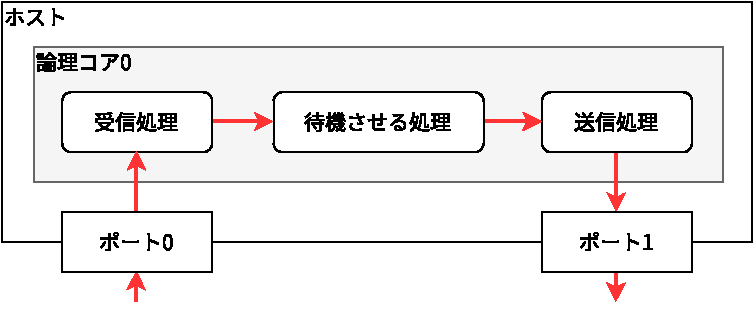
\includegraphics[width=\columnwidth]{pictures/PreExperimentOne.pdf}
  \caption{事前実験1用のプログラム}
  \label{fig:PreExperimentOne}
\end{figure}

\subsection{実験環境}
事前実験1で用いたネットワーク構成を図\ref{fig:PreExperimentNetwork}に示す.ホストAにおいてクライアントを動作させ,ホストBにおいて事前実験1用のプログラムを動作させた.クライアントには,DPDKベースのパケットジェネレータであるPktgen \cite{Pktgen} を用いた.事前実験1で用いた計算機の性能を表\ref{tab:MachineSpec},Pktgenの設定を表\ref{tab:PktgenSettings}に示す.

パケットはクライアントが動作するホストAのポート0から送信され,事前実験1用のプログラムが動作するホストBのポート0に到着する.到着したパケットは事前実験1用のプログラムによって待機させられてから,ホストBのポート1からホストAのポート1へと送り返される.

\begin{figure}[htb]
  \centering
  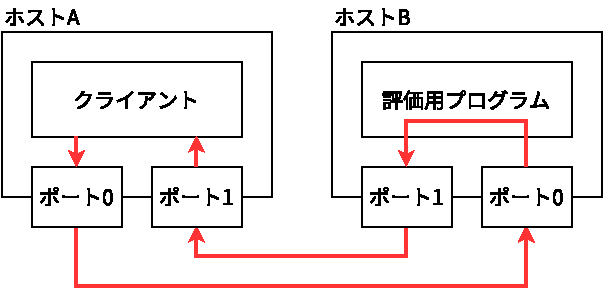
\includegraphics[width=\columnwidth]{pictures/PreExperimentNetwork.pdf}
  \caption{事前実験1で用いたネットワーク構成}
  \label{fig:PreExperimentNetwork}
\end{figure}

\begin{table}[htb]
  \centering
  \caption{事前実験1で用いた計算機の性能}
  \begin{tabular}{|c|c|} \hline
    OS     & Ubuntu 20.04                           \\ \hline
    CPU    & AMD Ryzen 5 3400G (4-cores, 8-threads) \\ \hline
    Memory & 16GB                                   \\ \hline
    NIC    & Intel X540-AT2 (10GbE, 2-ports)        \\ \hline
  \end{tabular}
  \label{tab:MachineSpec}
\end{table}

\begin{table}[htb]
  \centering
  \caption{Pktgenの設定}
  \begin{tabular}{|c|c|} \hline
    パケットのサイズ     & 64バイト, 128バイト \\ \hline
    送信するパケットの数 & 100,000,000パケット \\ \hline
    送信レート           & 100\%               \\ \hline
  \end{tabular}
  \label{tab:PktgenSettings}
\end{table}

\subsection{実験結果・考察}
事前実験1の結果を図\ref{fig:PreExperimentOneResult}に示す.このグラフの横軸はパケットの待機時間,縦軸は通信のスループットを表している.また,青はパケットサイズが64バイトのとき,赤はパケットサイズが128バイトのときの結果である.グラフより,パケットサイズが64バイトの場合,待機時間が1600ns以下のときスループットは一定であり,それを超えると単調減少することを確認した.また,パケットサイズが128バイトの場合,待機時間が3200ns以下のときスループットは一定であり,それを超えると単調減少することを確認した.よって,送信するパケットのサイズが小さく,送信レートが100\%という厳しい条件でも,処理時間が1600ns以下の計算処理であればスループットに影響を与えずにDPDKの送受信スレッドで実行できると考える.

\begin{figure}[htb]
  \centering
  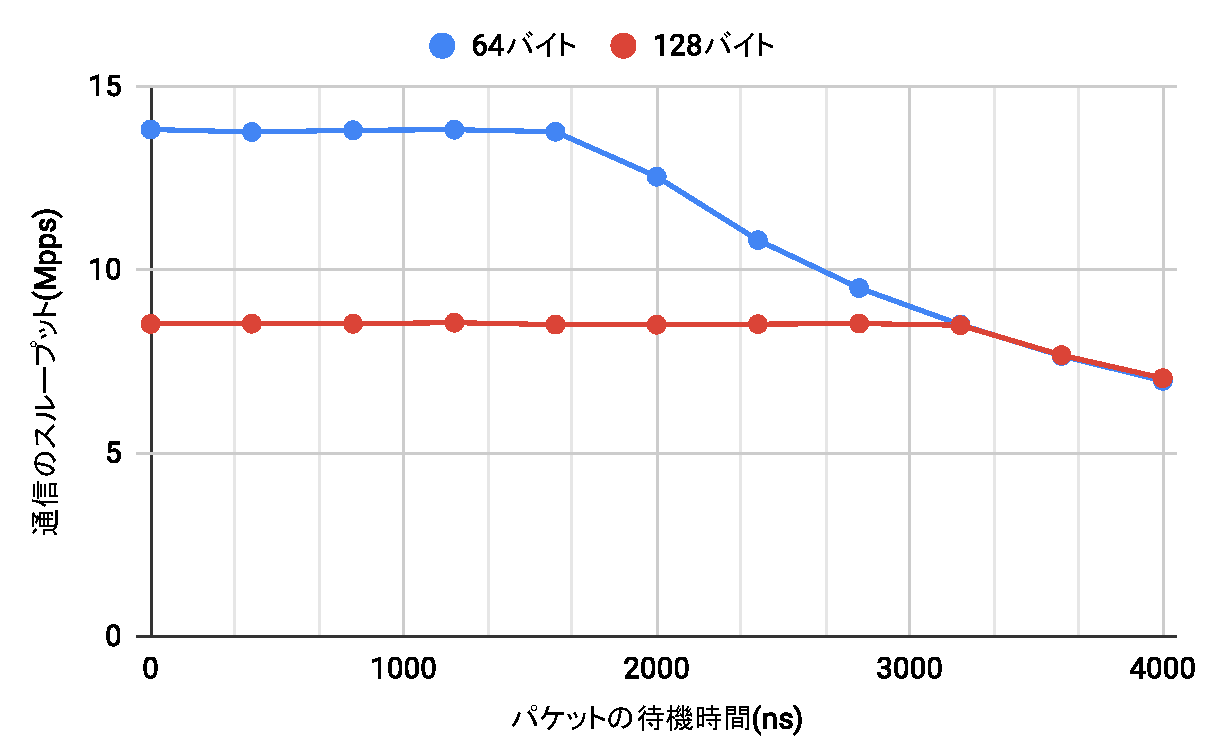
\includegraphics[width=\columnwidth]{pictures/PreExperimentOneResult.pdf}
  \caption{事前実験1の結果}
  \label{fig:PreExperimentOneResult}
\end{figure}
